\chapter{Cenni di teoria del suono} \label{chap:teoria_suono}
	
	\mylettrine{I}{ntuitivamente}, prima di poter parlare di algoritmi di compressione audio, e quindi di MP3, sarà necessario innanzitutto definire cos'è il suono e come si comporta. In questo capitolo verranno quindi presentati alcuni concetti fondamentali di teoria del suono, sia dal punto di vista fisico (onde e tutto ciò che ne concerne) che dal punto di vista informatico (campionamento e sintesi).
	
	\section{Il suono come onda} \label{sec:suono_onda}
		
		\begin{defi} \label{defi:suono}
			Il \emph{\textbf{suono}} è un'\emph{onda meccanica}, ovvero un'\emph{onda di pressione} che si propaga attraverso un mezzo.
		\end{defi}
		
		Questa definizione che abbiamo appena dato sul suono è molto chiara e concisa: il suono è un'onda. Ma non una qualsiasi onda. Il suono è un'onda di pressione, ovvero non è nient'altro se non l'oscillazione (movimento ``avanti-indietro'', in parole povere) del mezzo in cui si propaga, che può essere solido o fluido. Il timpano umano è infatti una membrana sottilissima volta a captare queste oscillazioni presenti attorno a noi; sarà poi il cervello che tradurrà i movimenti della membrana in informazioni utili, interpretandole come quello che noi chiamiamo suono.\\
		Come tutte le onde, anche il suono avrà quindi tutta una serie di attributi caratteristici, quali:
		\begin{itemize}
			\item \textbf{periodo}: minimo intervallo di tempo dopo il quale i valori dell'onda si ripetono ($s$, secondi);
			\item \textbf{frequenza}: numero di oscillazioni per unità di tempo ($Hz$, hertz);
			\item \textbf{lunghezza d'onda}: minima distanza dopo la quale  i valori dell'onda si ripetono($m$, metri);
			\item \textbf{numero d'onda}: numero di oscillazioni per unità di lunghezza ($m^{-1}$, metri alla meno uno);
			\item \textbf{ampiezza}: misura i cambiamenti dell'onda all'interno di uno stesso periodo (varia);
				\begin{itemize}
					\item \textit{ampiezza picco-a-picco}: massimo scarto tra una cresta (punto di massimo dell'onda) e la valle (punto di minimo) successiva;
					\item \textit{ampiezza a picco}: massimo valore assoluto dell'onda;
					\item \textit{ampiezza RMS} (root mean square): scarto quadratico medio dell'ampiezza.
				\end{itemize}
			\item \textbf{velocità}: velocità con cui l'onda si propaga nel mezzo ($\sfrac{m}{s}$, metri al secondo).
		\end{itemize}
		
		\begin{figure}[h!]
			\centering
				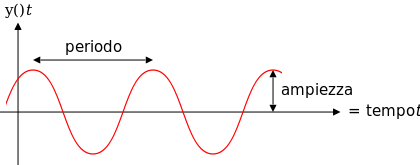
\includegraphics[scale=0.7]{periodo_ampiezza.png}
			\caption{Periodo e ampiezza di un'onda periodica.}
			\label{fig:periodo_ampiezza}
		\end{figure}
		
		\begin{figure}[h!]
			\centering
				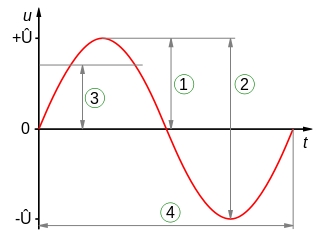
\includegraphics[scale=0.75]{ampiezze.png}
			\caption[Diversi tipi di ampiezze.]{Diversi tipi di ampiezze: ampiezza a picco (1), ampiezza picco-a-picco (2) e ampiezza RMS (3).}
			\label{fig:ampiezze}
		\end{figure}
		
		Come è facile dedurre, \textit{periodo} e \textit{frequenza} sono uno l'inverso dell'altro, come anche \textit{lunghezza d'onda} e \textit{numero d'onda}. L'unità di misura dell'ampiezza dipende dal tipo d'onda che si sta analizzando: se si tratta di corrente elettrica può rappresentare un voltaggio ($V$, volt), una corrente ($A$, ampere) o la potenza ($W$, watt), mentre se parliamo di onde sonore l'ampiezza può rappresentare la forza dell'onda di pressione (\textit{dB}, decibel), oppure il movimento oscillatorio stesso, con 0 punto di quiete e -1 ed 1 limiti, rispettivamente, inferiore e superiore. La velocità d'onda è invece calcolata come $v=\sfrac{\lambda}{p}=\lambda\cdot f$, dove $\lambda$ è la lunghezza d'onda, $p$ il suo periodo ed $f$ la sua frequenza. La velocità del suono a 20 ${}^\circ C$ nell'aria al livello del mare è circa 343 $\sfrac{m}{s}$, ma come per molte altri tipi di onda la sua velocità varia a seconda di molti fattori, come natura del mezzo, temperatura, densità, ecc\dots.
	
	\section{Percezione del suono} \label{sec:percezione}
	
		Avendo definito il suono come un'onda, possiamo affermare che in natura esistono un'infinità di suoni diversi, generati da altrettante frequenze caratteristiche. L'orecchio umano, tuttavia, non è in grado di percepire tutte le frequenze esistenti in natura: in generale, l'uomo riesce a percepire tutte le frequenze che vanno dai 20 \textit{Hz} ai 20 \textit{kHz} (20mila \textit{Hz}). Ovviamente, ci sono eccezioni e casi particolari di persone che affermano di riuscire a percepire e distinguere anche frequenze al di fuori di questo range. Inoltre, l'uomo non percepisce tutte le frequenze allo stesso modo: più ci si avvicina ai limiti del range di udibilità, più sarà difficile percepire tale suono. Infatti le frequenze che meglio possiamo sentire sono quelle tra i 2 e i 4 \textit{kHz} \cite{raissi}.\\
		A tal proposito, la Figura \ref{fig:ath} rappresenta la \textit{soglia assoluta di udibilità} (in inglese, \textit{absolute threshold of hearing}) per un uomo medio a 20, 40 e 60 anni, ovvero qual'è la minima intensità che ogni frequenza deve avere per essere percepita dall'uomo. In altre parole, tutto ciò che l'uomo non sente è rappresentato dall'area sottesa dal grafico in Figura \ref{fig:ath}.
		
		\begin{figure}[h!]
			\centering
				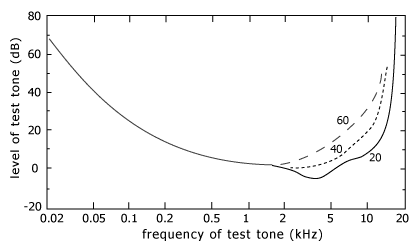
\includegraphics[scale=1]{ath.png}
			\caption[Soglia assoluta di udibilità.]{Soglia assoluta di udibilità per un uomo medio a 20, 40 e 60 anni.}
			\label{fig:ath}
		\end{figure}
		
		L'uomo, quindi, non è una macchina, in quanto il suo orecchio e il suo cervello non sono strumenti perfetti. È nata infatti negli anni la disciplina detta \textit{psicoacustica}, che si occupa di studiare non tanto il suono in sé dal punto di vista fisico, ma come esso viene percepito dall'uomo. Della psicoacustica sentiremo parlare più avanti quando entreremo nel merito dell'MP3, in quanto essa costituisce uno dei principi cardine che stanno alla base della tecnologia MP3.
		
	\section{Sintesi e Campionamento} \label{sec:campionamento_sintesi}
	
		Abbiamo detto che il suono è un'onda di pressione, ovvero il movimento oscillatorio (``avanti-indietro'') del mezzo nel quale si propaga. Infatti tutti i suoni sono prodotti dal movimento, più o meno rapido, di uno o più corpi, il quale genera questa catena di oscillazioni, producendo il suono stesso.
		
		\subsection{Sintesi} \label{subsec:sintesi}
		
			Come viene riprodotto, allora, artificialmente un suono? Secondo quanto detto, abbiamo bisogno di un corpo che faccia a comando questo movimento oscillatorio. Non solo, è necessario anche che il movimento ``avanti-indietro'' che questo corpo esegue abbia la stessa frequenza del suono che vogliamo riprodurre, ovvero che esegua lo stesso numero di oscillazioni nell'unità di tempo.\\
			\\
			L'oggetto di cui stiamo parlando è detto \textit{speaker}, o più comunemente \textit{altoparlante}. Uno speaker è formato da un elettromagnete che, a seconda dell'intensità della corrente elettrica che lo attraversa, si sposterà avanti o indietro rispetto alla posizione di quiete. La gestione dello speaker avviene tramite una \textit{scheda audio} (o \textit{soundcard} in inglese), ovvero un DAC (\textit{Digital-to-Analog Converter}) che trasforma un numero digitale in input in un segnale elettrico in output. Se si utilizza la convenzione prima esposta (0 = stato di quiete, -1 = tutto indietro, 1 = tutto avanti) possiamo allora fornire alla scheda audio una serie di valori nel tempo, in modo da far muovere lo speaker avanti e indietro. Se rappresentassimo questo movimento in funzione del tempo, otterremmo proprio i ben noti grafici delle onde sonore, come quelli nelle Figure \ref{fig:periodo_ampiezza} e \ref{fig:ampiezze}. Ad esempio per riprodurre la nota La, che ha una frequenza di 440 \textit{Hz} \cite{mtu}, lo speaker dovrà eseguire 440 oscillazioni ``avanti-indietro'' ogni secondo.
			
		\subsection{Campionamento} \label{subsec:campionamento}
		
		\begin{figure}[h!]
			\centering
				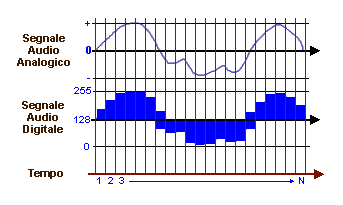
\includegraphics[scale=1]{campione.png}
			\caption{Campionamento di un segnale audio analogico.}
			\label{fig:campione}
		\end{figure}
		
		Si osservi che, per quanto detto prima, per oscillazione si intende un intero movimento ``avanti-indietro'', ovvero un intero periodo, quindi affinché il suono della nota La venga prodotto correttamente, lo speaker dovrà effettuare 440 movimenti in avanti e 440 movimenti indietro e sarà quindi necessario fornire alla scheda audio l'informazione su questi 880 movimenti totali. Il fatto di richiedere il doppio di informazione rispetto al numero di oscillazioni al secondo è noto come \textit{Teorema del campionamento di Shannon-Nyquist}. Prima di parlare di questo importante teorema, introduciamo due concetti chiave del campionamento:
		
		\begin{defi} \label{defi:sampling_frequency}
			La \emph{\textbf{sampling frequency}} (o \emph{frequenza di campionamento}) è il numero di volte in cui viene misurato (o campionato) un segnale audio esterno in un determinato intervallo di tempo.
		\end{defi}
		
		\begin{defi} \label{defi:bit_depth}
			La \emph{\textbf{bit depth}} (o \emph{profondità di bit}) indica il numero di bit riservati alla memorizzazione di ogni campione (o sample).
		\end{defi}
		
		Un microfono, in linea di massima, è sostanzialmente un altoparlante al contrario: una membrana collegata ad un elettromagnete si muove secondo i suoni esterni, assecondandone i movimenti. Ogni $\sfrac{1}{f}$ secondi (con $f$ frequenza di campionamento) viene misurata la posizione di questa membrana rispetto alla posizione di quiete. Questa misura prende il nome di \textit{campione} (o \textit{sample}) e ognuno di questi campioni verrà registrato in memoria utilizzando un numero di bit definito dalla bit depth. Una volta registrati abbastanza campioni, effettuare la sintesi tramite scheda audio e speaker sarà semplice: verrà effettuata una semplice interpolazione tra i sample registrati e i valori della funzione risultante verrano dati in pasto alla scheda audio, che azionerà lo speaker di conseguenza.\\
		Ovviamente, una maggiore sampling frequency permette di avere campionamenti più fitti e quindi una riproduzione più accurata del suono registrato. Analogamente, più bit si riservano per i campioni, minore sarà l'errore commesso su ogni misura (detto \textit{errore di quantizzazione}), rendendo ancora una volta la registrazione più accurata. Tuttavia, avere più sample e/o avere sample più voluminosi (come quantità di bit) andrà a incidere negativamente sulle dimensioni totali della registrazione risultante, rendendo, in casi estremi, il file finale eccessivamente grande.\\
		Possiamo quindi trovare un compromesso tra dimensioni del file e qualità audio? Come vedremo più avanti, il punto di forza dell'MP3 sta proprio nell'aver definito un modo di memorizzare i file audio che permetta sia di godere di un'ottima qualità audio che, allo stesso tempo, di mantenere le dimensioni del file ridotte.\\
		
		\begin{figure}[h!]
			\centering
				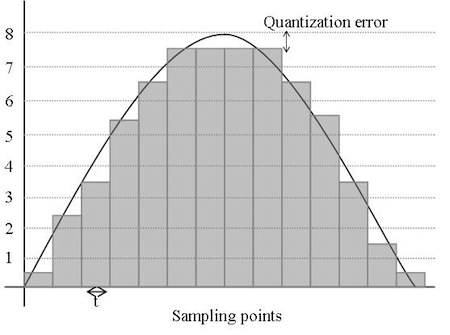
\includegraphics[scale=1]{quantization.jpg}
			\caption{Campionamento ed errore di quantizzazione.}
			\label{fig:quantization}
		\end{figure}
		
		\begin{figure}[h!]
			\centering
				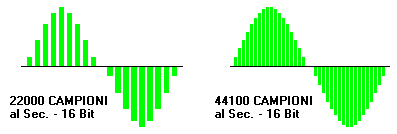
\includegraphics[scale=1]{sampling_22_441.png}
			\caption[Uso di differenti sample frequency.]{Uso di differenti sampling frequency: all'aumentare della sampling frequency aumenta la fedeltà del file audio ma anche le dimensioni complessive.}
			\label{fig:sampling_22_441}
		\end{figure}
		
		Il Teorema del campionamento di Shannon-Nyquist serve a mettere in relazione la frequenza di campionamento con la frequenza di output ottenuta dalla sintesi:
		
		\begin{teo}[Shannon-Nyquist] \label{teo:shannon_nyquist}
			Per poter correttamente riprodurre un segnale audio, come minimo devono essere misurati due campioni per ogni periodo della sua onda caratteristica.
		\end{teo}
		
		Quindi come dicevamo prima, se vogliamo correttamente riprodurre una nota La (440 \textit{Hz}), avremmo bisogno di una frequenza di campionamento di almeno 880 \textit{Hz}. Viceversa, campionando con una frequenza fissata, non sarà possibile riprodurre tutte le frequenze maggiori della metà della sampling frequency (noto come \textit{limite di Nyquist}).\\
		La ``qualità CD'', infatti, è caratterizzata da una sampling frequency di 44.1 \textit{kHz}, il che significa che verranno scartate tutte le frequenze al di sopra dei 22.05 \textit{kHz}. Questo valore non è casuale: 22.05 \textit{kHz} è poco sopra il limite superiore di udibilità dell'uomo (20 \textit{kHz}). In parole povere, registrare frequenze più alte sarebbe soltanto uno spreco di spazio, in quanto non verrebbero comunque udite dall'uomo.\\
		\\
		Se la frequenza di campionamento non è abbastanza elevata, alcuni campioni si potrebbero sovrapporre in frequenza, dando origine al fenomeno (negativo) detto \textit{aliasing}: l'aliasing rende impossibile ricostruire parte del segnale originale a partire dai suoi campioni (come formalizzato dal Teorema di Shannon-Nyquist). L'aliasing si elimina aumentando la frequenza di campionamento. Se il segnale di input non è a banda limitata, allora si filtra prima attraverso un filtro passa-basso, detto \textit{filtro anti-aliasing}.